%%%%%%%%%%%%%%%%%%%%%%%%%%%%%%%%%%%%%%%%%%%%%%%%%%%%%%%%%%%%%

\mainmatter
\setcounter{page}{1}

\lectureseries[\course]{\course}

\auth[\lecAuth]{Lecturer: \lecAuth\\ Scribe: \scribe}
\date{January 7, 2010}

\setaddress

% the following hack starts the lecture numbering at 1
\setcounter{lecture}{1}
\setcounter{chapter}{1}

\lecture{Course Introduction}

\section{Limit Cycles Recap}
Last lecture we studied linear and nonlinear limit cycles. An example of a linear limit cycle is a  harmonic oscillator given by
$$\ddot{x} + x = 0$$
and the state space is shown in Figure \ref{fig:02secondorder}.

\begin{figure}[ht!]
	\centering
	\includegraphics[width=.4\textwidth]{images/01secondorder}
	\caption{Limit cycle for second order harmonic oscillator.}
	\label{fig:02secondorder}
\end{figure}

An example of a nonlinear limit cycle is a Van der Pol oscillator given by
$$\ddot{x} + (x^2-1)\ddot{x} + x = 0$$
and the state space is shown in Figure \ref{fig:02vdplc}. Note that there is positive damping for $|x|>1$ and negative damping for $|x|<1$.

\begin{figure}[ht!]
	\centering
	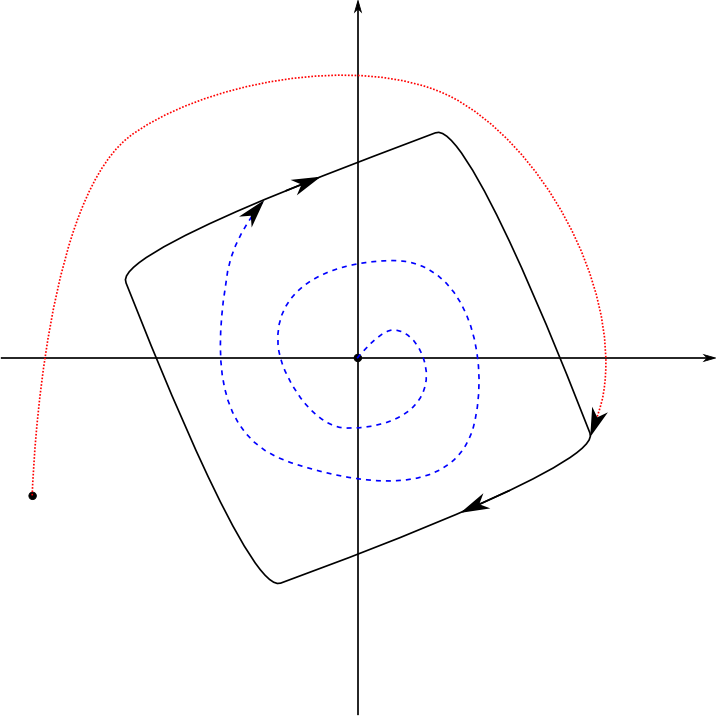
\includegraphics[width=.4\textwidth]{images/02vdplc}
	\caption{Limit cycle for Van der Pol oscillator.}
	\label{fig:02vdplc}
\end{figure}

The harmonic oscillator has a period of $2\pi$ and the Van der Pol oscillator has a base harmonic accompanied by lower frequencies and can be modeled using a Fourier series.

\subsection{Isolated Periodic Orbit}
An isolated periodic orbit will have a single amplitude. Examples of Van der Pol oscillators are
\begin{itemize}
\item The human heart.
\item An LC circuit with a tunnel diode.
\item A compressor in ``surge'' mode where there is a pumping motion in flow and pressure as found in jet engines.
\end{itemize}

\section{Chaos}
Chaotic systems are ``random'' yet created by a deterministic system like $\dot{x}=f(x)$. It is interesting to look at the lowest order autonomous systems that can generate chaotic behavior which have been found to be of order $n=3$ in continuous time and order $n=1$ in discrete time. In this course we will be studying continuous time for the most part as it is more relevant to mechanical and aerospace systems than discrete time is.

\subsection{Lorenz Equations}
The Lorenz equations given in (\ref{eq:02lorenz}) are an example of chaotic dynamics in continuous time. The equations are not periodic and cannot be represented by a Fourier series.
\begin{align}
\label{eq:02lorenz}
\dot{x} &= \sigma(y - x) \nonumber \\
\dot{y} &= \rho x - y - xz \\
\dot{z} &= -\beta z + xy \nonumber
\end{align}
where $(x,y,z)\in\mathbb{R}^3$ and $\sigma, \rho, \beta > 0$.

To find the equilibria of the Lorenz equations we set $\dot{x}=f(x)=0$ and solve the set of ODEs in (\ref{eq:02lorenz}) to find
\begin{align*}
\dot{x} &= \sigma(y-x) = 0 \Rightarrow y = x \\
\dot{z} &= -\beta z + xy = 0 \Rightarrow z = \frac{y^2}{\beta} \\
\dot{y} &= \rho x-y-xz = 0 \Rightarrow (\rho-1)y - y\frac{y^2}{\beta} = 0 \Rightarrow y = 0, \pm\sqrt{\beta(\rho-1)}
\end{align*}
which yields the equilibria as
\begin{align*}
(x,y,z) = \begin{cases} (0,0,0) \\ (\sqrt{\beta(\rho-1)}, \sqrt{\beta(\rho-1)}, \rho-1) \\ (-\sqrt{\beta(\rho-1)}, -\sqrt{\beta(\rho-1)}, \rho-1) \end{cases}
\end{align*}

\section{Qualitative Behavior Near Equilibria}
This section corresponds to \S2.3 of Khalil. Let
$$\dot{x} = f(x), \qquad f(p) = 0$$
so that the point $p$ is an equilibria. We can use a Taylor series expansion about $x=p$ to find
\begin{align*}
\dot{x} = \underbrace{f(p)}_{=0} + \underbrace{\left.\frac{\partial f(x)}{\partial x}\right|_{x=p}}_{\text{constant square matrix}} \underbrace{(x-p)}_{y} + \text{H.O.T.}
\end{align*}
Let
$$A \triangleq \left.\frac{\partial f(x)}{\partial x}\right|_{x=p}$$
and then the linearization is $\dot{y}=Ay$. Note that
\begin{align*}
\frac{\partial f(x)}{\partial x} = \left[\begin{array}{c c c} \frac{\partial f(x_1)}{\partial x_1} & \cdots & \frac{\partial f(x_1)}{\partial x_n} \\ \vdots & \ddots & \vdots \\ \frac{\partial f(x_n)}{\partial x_1} & \cdots & \frac{\partial f(x_n)}{\partial x_n} \end{array}\right]
\end{align*}

For second order systems the state space is the plane spanned by $x_1 = x$ and $x_2 = \dot{x}$ as we have seen in several previous examples.

\subsection{Qualitative Behavior of Second-Order Linear Systems}
For the system
$$\dot{x} = Ax$$
we have to look at the eigenvalues and eigenvectors of $A$. There are three possible Jordan forms of $A$ given as
\begin{align*}
\left[\begin{array}{c c} \lambda_1 & 0 \\ 0 & \lambda_2 \end{array}\right], \qquad
\left[\begin{array}{c c} \alpha & -\beta \\ \beta & \alpha \end{array}\right], \qquad
\left[\begin{array}{c c} \lambda & k \\ 0 & \lambda \end{array}\right]
\end{align*}

In the first case we have $\lambda_1\neq\lambda_2\neq0$. Figure \ref{fig:02stable1} shows the stable mode for $\lambda_1, \lambda_2<0$, Figure \ref{fig:02unstable1} shows the unstable mode for $\lambda_1, \lambda_2>0$ and Figure \ref{fig:02saddle1} shows the saddle point for $\lambda_1>0$ and $\lambda_2<0$.

\begin{figure}[ht!]
  \centering
  \subfloat[$\lambda_1,\lambda_2<0$, stable mode.]{
    \label{fig:02stable1}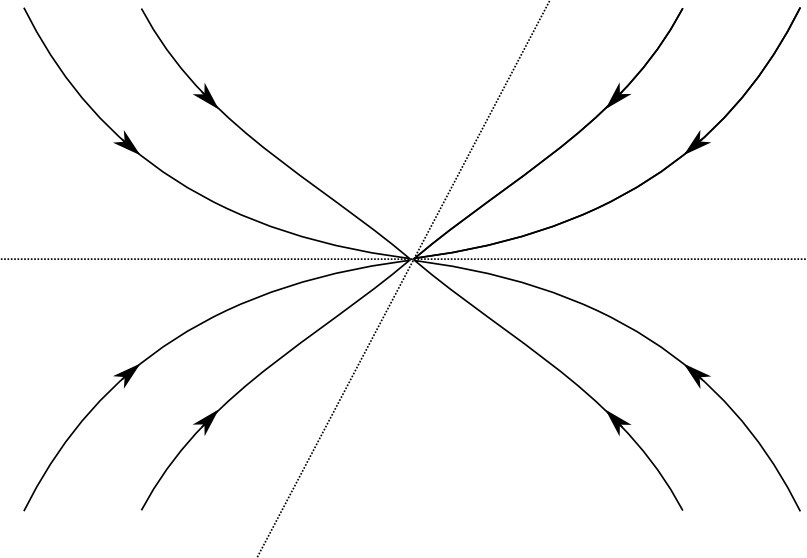
\includegraphics[width=0.35\textwidth]{images/02stable1}
  } \hfill
  \subfloat[$\lambda_1,\lambda_2>0$, unstable mode.]{
    \label{fig:02unstable1}\includegraphics[width=0.35\textwidth]{images/02unstable1}
  } \\
  \subfloat[$\lambda_1>0,\lambda_2<0$, saddle point.]{
    \label{fig:02saddle1}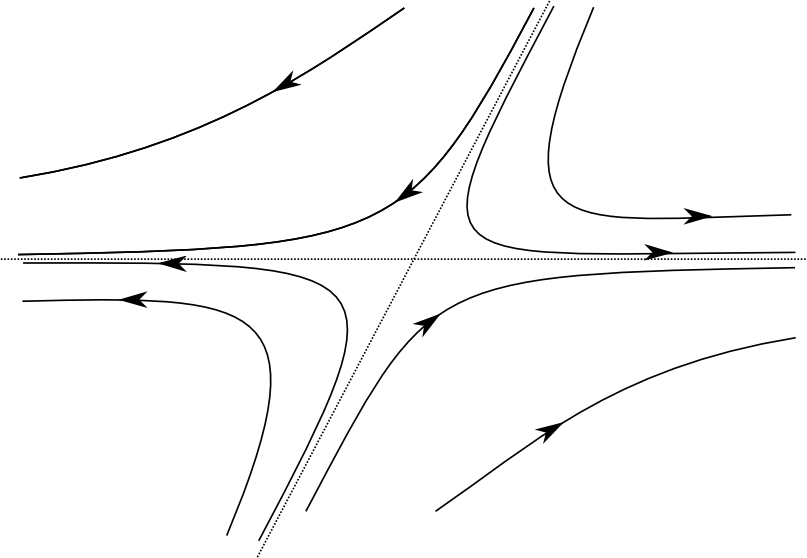
\includegraphics[width=0.35\textwidth]{images/02saddle1}
  }
  \caption{Case 1: $\lambda_1\neq\lambda_2\neq0$.}
  \label{fig:02case1}
\end{figure}

In the second case we have $\lambda_{1,2}=\alpha\pm\ j\beta$. Figure \ref{fig:02stable2} shows the stable mode for $\alpha<0$, Figure \ref{fig:02unstable2} shows the unstable mode for $\alpha>0$ and Figure \ref{fig:02center2} shows the oscillatory behavior that occurs when $\alpha=0$.

\begin{figure}[ht!]
  \centering
  \subfloat[$\alpha<0$, stable mode.]{
    \label{fig:02stable2}\includegraphics[width=0.35\textwidth]{images/02stable2}
  } \hfill
  \subfloat[$\alpha>0$, unstable mode.]{
    \label{fig:02unstable2}\includegraphics[width=0.35\textwidth]{images/02unstable2}
  } \\
  \subfloat[$\alpha=0$, center point.]{
    \label{fig:02center2}\includegraphics[width=0.35\textwidth]{images/02center2}
  }
  \caption{Case 2: $\lambda_{1,2} = \alpha\pm j\beta$.}
  \label{fig:02case2}
\end{figure}

In the third case we have $\lambda_1=\lambda_2=\lambda\neq0$ and we can have $k=0$ or $k=1$. If $k=0$ then there are two independent eigenvectors and Figure \ref{fig:02lltwo3} shows the stable mode for $\lambda<0$ and Figure \ref{fig:02lgtwo3} shows the unstable mode for $\lambda>0$. When $k=1$ there is only a single independent eigenvector and troublesome behavior exists. Figure \ref{fig:02llone3} shows what happens when $\lambda<0$ and Figure \ref{fig:02lgone3} shows what happens when $\lambda>0$.

\begin{figure}[ht!]
  \centering
  \subfloat[$\lambda<0$, two independent eigenvectors.]{
    \label{fig:02lltwo3}\includegraphics[width=0.35\textwidth]{images/02lltwo3}
  } \hfill
  \subfloat[$\lambda>0$, two independent eigenvectors.]{
    \label{fig:02lgtwo3}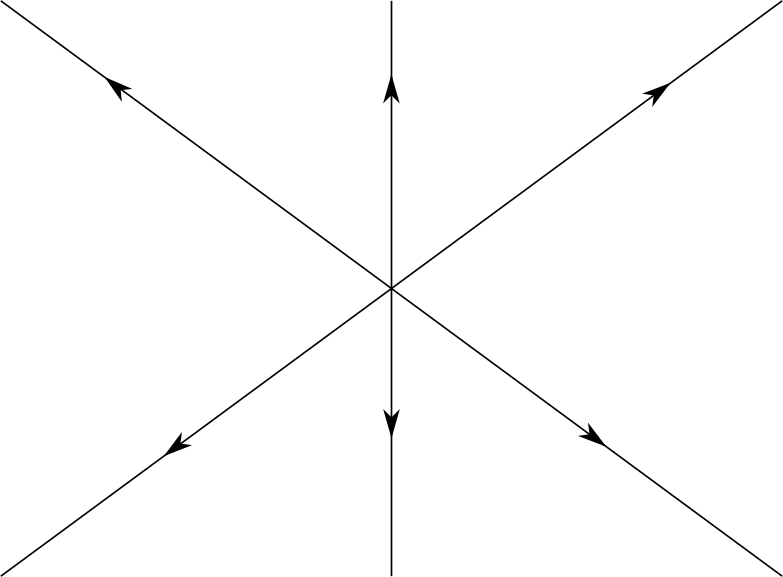
\includegraphics[width=0.35\textwidth]{images/02lgtwo3}
  } \\
  \subfloat[$\lambda<0$, one independent eigenvector.]{
    \label{fig:02llone3}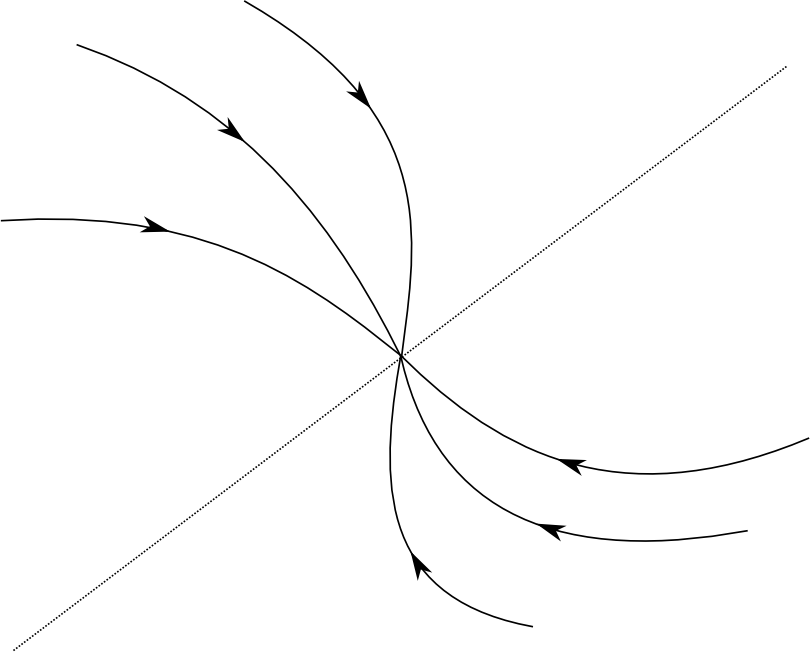
\includegraphics[width=0.35\textwidth]{images/02llone3}
  } \hfill
  \subfloat[$\lambda>0$, one independent eigenvector.]{
    \label{fig:02lgone3}\includegraphics[width=0.35\textwidth]{images/02lgone3}
  }
  \caption{Case 3: $\lambda_1=\lambda_2=\lambda\neq0$.}
  \label{fig:02case2}
\end{figure}
%%%%%%%%%%%%%%%%%%%%%%%%%%%%%%%%%%%%%%%%%%%%%%%%%%%%%%%%%%%%%